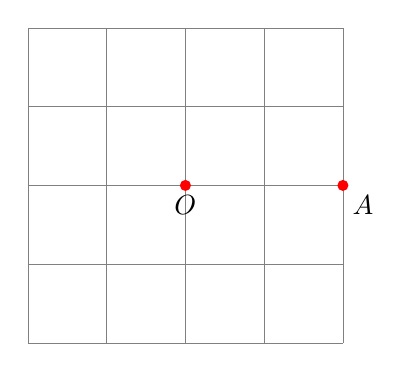
\begin{tikzpicture}
  \draw[help lines] (-2,-2) grid (2,2);
  \coordinate (O) at (0,0);
  \coordinate (A) at +(0:2);  % 圆上一点, 相对坐标
  \draw[thick,circle={O,A}];
  \foreach \p in {O,A}
    \fill[red] (\p) circle (2pt);
  \draw (O) node[below] {$O$};
  \draw (A) node[below right] {$A$};
\end{tikzpicture}